\chapter{TINJAUAN PUSTAKA}
\vspace{1ex}

\section*{}
Demi mendukung penelitian ini, dibutuhkan beberapa teori penunjang sebagai bahan acuan dan referensi. Dengan demikian penelitian ini menjadi lebih terarah. 
\vspace{1ex}

\section{Machine Learning}
\vspace{1ex}

\begin{figure} [!htb]
	\captionsetup{justification=centering}
	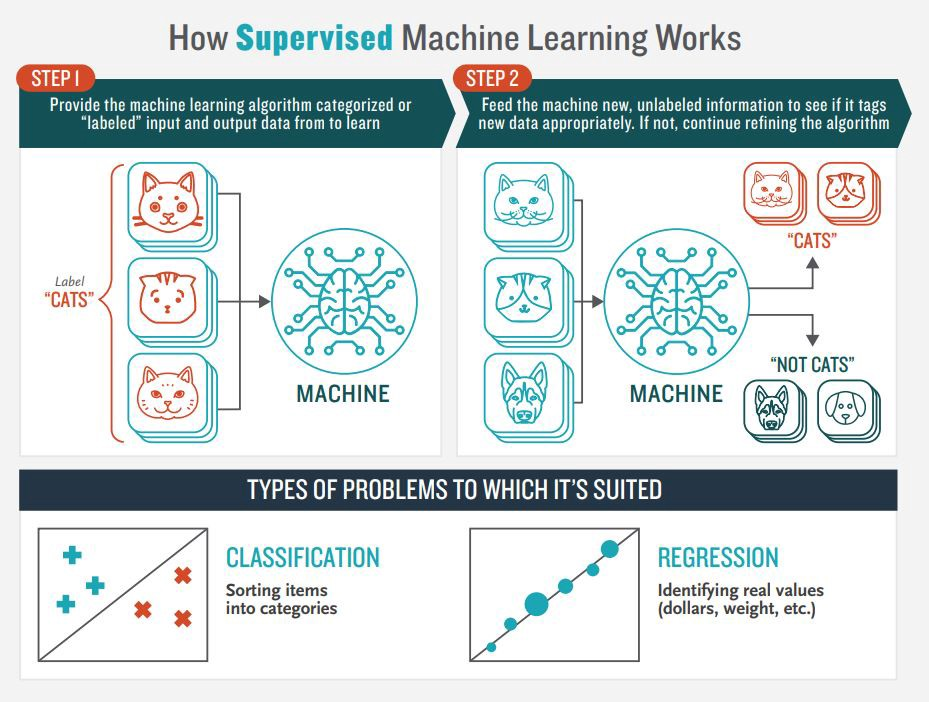
\includegraphics[scale=0.2]{img/supervised.jpeg}
	\caption{Cara Kerja Supervised Learning\cite{cit:8}}
	\label{fig:2.1}
\end{figure}

\textit{Machine learning} atau pembelajaran mesin adalah suatu cabang teknologi yang menerapkan penggunaan \textit{artificial intelligence}. \textit{Machine learning} pertama kali diperkenalkan oleh Thomas Bayes, Adrien-Marie Legendre, dan Andrey Markov pada sekitar tahun 1920\cite{cit:7}. Dengan menggunakan fundamental \textit{Machine Learning} yang diciptakan oleh ilmuwan - ilmuwan tersebut, \textit{Artificial Intelligence} kini dapat berkembang sampai dapat mengalahkan pemain catur profesional.
\vspace{1ex}

\par Dengan berkembangnya \textit{machine learning}, tugas-tugas yang dilakukan oleh \textit{machine learning} ini pun semakin beragam. Beberapa contoh dari tugas-tugas yang dapat dilakukan oleh \textit{Machine Learning} adalah validasi data, menemukan pola-pola tertentu dari sumber data yang besar, mengklasifikasi grup dan objek berdasarkan kesamaan pola.

\vspace{1ex}
\par \textit{Supervised learning} jika diartikan secara harfiah adalah pembelajaran yang ada supervisornya. Disini supervisi dilakukan oleh orang yang melakukan training kepada label di setiap datanya. Sebagai contoh dapat dilihat pada gambar 2.1. 
\vspace{1ex}

\par Pada gambar diatas, masing-masing gambar kucing diberi label “CATS” dan yang bukan kucing (“anjing”,”beruang”,”lain-lain”) diberi label “NOT CATS”. Ketika gambar baru dimasukkan setiap label akan dicompare sampai selesai, dan yang memiliki persentase lebih banyak akan diambil sebagai prediksi akhir.

\vspace{1ex}

\par Pada pendekatan \textit{supervised learning}, terdapat input dan output yang dapat dibuat menjadi hubungan matematis.\textit{Supervised learning} cocok untuk digunakan untuk memprediksi dimana sudah ada contoh data yang lengkap, sehingga pola yang terbentuk adalah hasil pembelajaran dari data lengkap tersebut. Beberapa algoritma yang termasuk dalam \textit{supervised learning} adalah sebagai berikut:
\begin{enumerate}
	\vspace{-2mm}
	\item Regresi Linier Berganda
	\vspace{-2mm}
	\item Analisis Deret Waktu
	\vspace{-2mm}
	\item \textit{Decision Tree} dan \textit{Random Forest}
	\vspace{-2mm}
	\item \textit{Naive Bayes Classifier}
	\vspace{-2mm}
	\item \textit{Nearest Neighbor Classifier}
	\vspace{-2mm}
	\item \textit{Artificial Neural Network}
	\vspace{-1mm}
\end{enumerate}
\par Jika dibandingkan dengan \textit{supervised learning}, \textit{unsupervised learning} tidak membutuhkan adanya label sebagai dasar prediksi melainkan menggunakan kesamaan atribut - atribut yang dimiliki oleh data tersebut. Jika atribut - atribut tersebut memiliki kesamaan maka data tersebut akan di \textit{cluster} menjadi satu. Sebagai contoh dapat dilihat pada gambar di bawah :

\begin{figure}[h!]
	\centering
	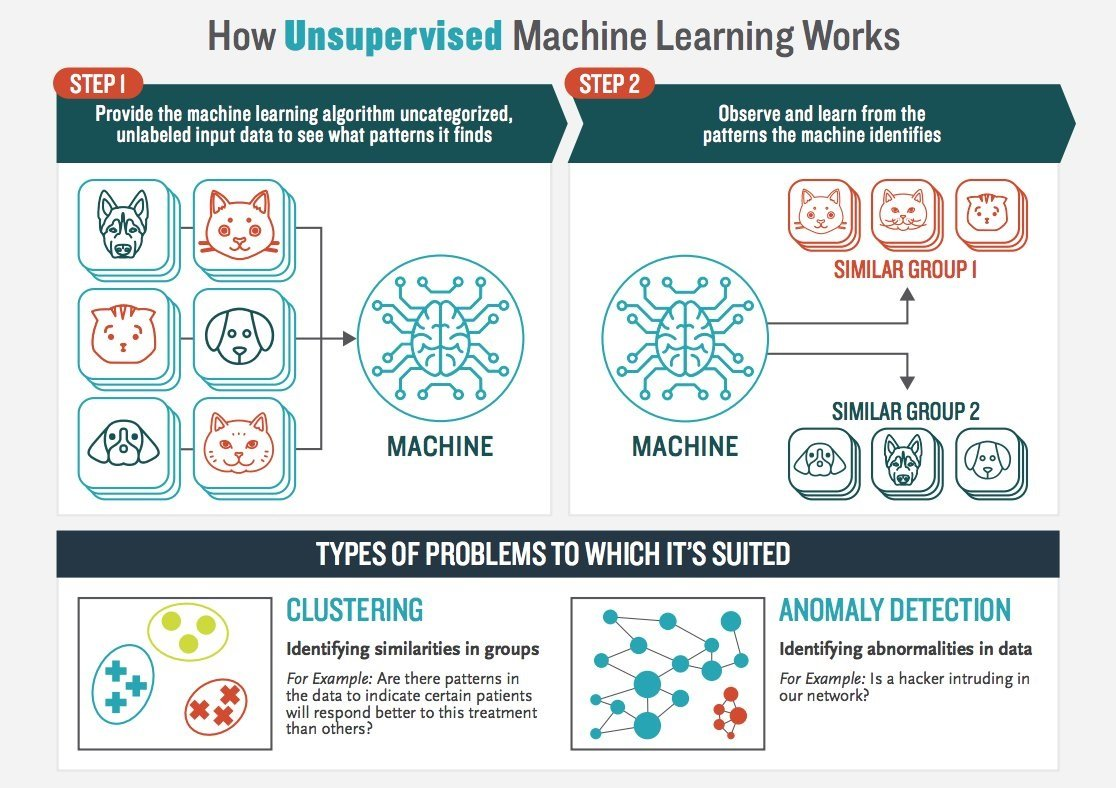
\includegraphics[scale=0.18]{img/unsupervised.jpg}
	\caption{Cara kerja Unsupervised Learning \cite{cit:8}}
	\label{fig:Unsupervised}
\end{figure}

\pagebreak

\par Pada Gambar 2.2 dapat dilihat bahwa disediakan gambar- gambar yang tidak memiliki label ke algoritma \textit{machine learning}. Setelah itu \textit{artificial intelligence} akan memisahkan gambar mana yang memiliki kesamaan di dalam \textit{cluster}. \textit{Cluster} yang ada merupakan hasil akhir klasifikasi yang dilakukan.

\par Namun \textit{unsupervised learning} tidak memiliki hasil spesifik layaknya pada \textit{supervised learning}. Hal ini dikarenakan tidak adanya label dasar (ground truth). Beberapa algoritma yang digunakan di \textit{unsupervised learning} :
\begin{enumerate}
	\vspace{-2mm}
	\item \textit{Clustering}
	\vspace{-2mm}
	\item \textit{Anomaly Detection}
	\vspace{-2mm}
	\item \textit{Training Model}
	\vspace{-2mm}
	\item \textit{Association Discovery}
\end{enumerate}

\vspace{1ex}

\par \textit{Deep learning} (Pembelajaran Dalam) merupakan bagian yang dalam dari \textit{machine learning} yang terdiri dari pemodelan fungsi yang ditata berlapis dan mendalam dengan menggunakan \textit{Artificial Neural Network} (ANN). ANN merupakan sebuah teknik atau pendekatan pengolahan informasi yang terinspirasi oleh cara kerja sistem saraf biologis, khususnya pada sel otak manusia dalam memproses informasi. Jenis pembelajaran dalam deep learning berupa \textit{supervised, semi-supervised}, dan \textit{unsupervised}.Deep learning dapat diimplementasikan dalam pengenalan citra, pengenalan suara, klasifikasi teks, dan sebagainya. 

\begin{figure}[h!]
\centering
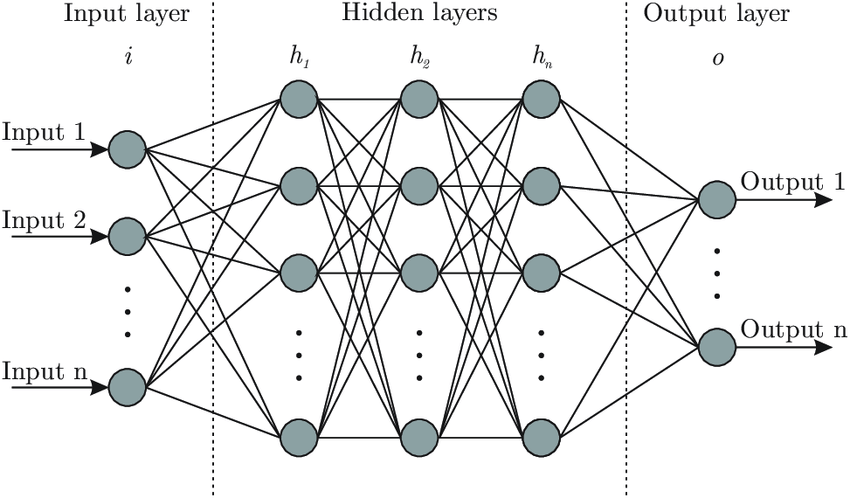
\includegraphics[scale=0.2]{img/Artificial.png}
\caption{Bentuk Artificial Neural Network \cite{cit:18}}
\label{fig:ANN}
\end{figure}

\section{\textit{Residual Network}}
\vspace{1ex}

\textit{Residual Neural Network} atau \textit{ResNet} merupakan sebuah \textit{Artificial Neural Network} (ANN) yang dibuat berdasarkan bentuk korteks serebral milik manusia. \textit{Residual Network} melakukan hal ini dengan memperkenalkan \textit{skip connection} atau \textit{shortcut}, dimana model dapat melompat dua atau tiga \textit{layer} jika memang hal tersebut merupakan hasil terbaik. Sebelum adanya model \textit{Residual Neural Network} penambahan layer pada suatu model hanya akan meningkatkan akurasi sampai suatu batas tertentu, sehingga penambahan layer setelah 20 hanya menambahkan kompleksitas model bukannya akurasi. Namun pada penelitian \textit{Deep Residual Learning for Image Recognition} yang dibuat oleh Kaiming He pada tahun 2015 memproposikan sebaliknya, apabila layer tambahan yang ada dapat mempelajari matriks identitas, maka minimal akurasi yang didapat pada \textit{layer} akan sama dengan apabila tidak menambahkan \textit{layer}. Untuk membuktikan hal tersebut dibuatlah sistem \textit{skip connection} atau \textit{shortcut} sehingga model dapat mempelajari matriks identitas dengan lebih mudah. Dari penelitian yang dilakukan pada dataset \textit{ImageNet}, \textit{Residual Network} dapat mengurangi \textit{loss} yang didapat ketika menambahkan lebih banyak \textit{layer} pada \textit{Artificial Neural Network} yang dibuat. \cite{cit:10}

\begin{figure}[h!]
	\centering
	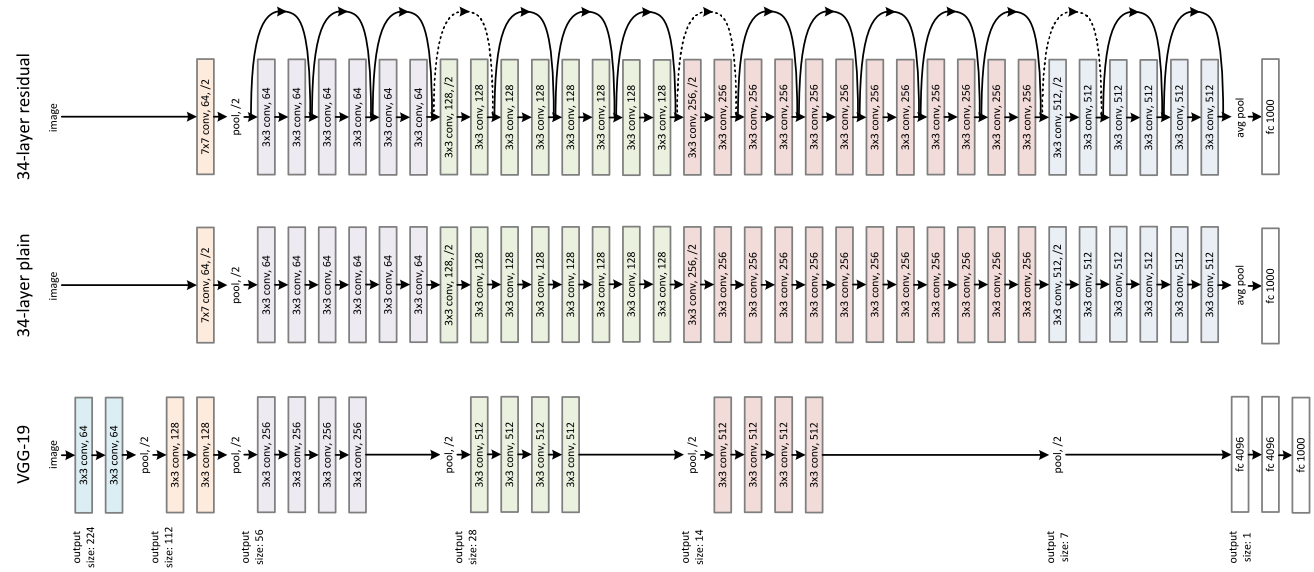
\includegraphics[scale=0.2]{img/ResNet.png}
	\caption{Perbandingan layer ResNet, plain, dan VGG-19 \cite{cit:10}}
	\label{fig:Resnet}
\end{figure}

\section{Pytorch}
\vspace{1ex}

\textit{Pytorch} merupakan sebuah library \textit{deep learning} pada \textit{Python} untuk menggantikan \textit{NumPy} dikarenakan membutuhkan kekuatan komputasi milik \textit{Graphics Processing Unit} (GPU). \textit{Library Pytorch} menyediakan fleksibilitas dan kecepatan komputasi maksimal ketika melakukan penelitian \textit{deep learning}. \textit{Pytorch} menyediakan \textit{pre-trained weights} dari model yang digunakan untuk mengklasifikasikan permasalahan lain sehingga dapat digunakan untuk mengurangi waktu dan kekuatan komputasi yang dibutuhkan. \cite{cit:11}
\vspace{1ex}

\section{\textit{Triplet Loss}}
\vspace{1ex}

\par \textit{Triplet Loss} merupakan sebuah \textit{Loss Function} yang umumnya digunakan dalam proses Re-Identifikasi. Pada fungsi ini dilakukan perbandingan jarak antara titik acuan terhadap titik positif yang merupakan gambar dalam kelas sama, dan perbandingan dengan titik negatif yang berasal dari kelas berbeda. Fungsi ini memastikan bahwa jarak ke titik positif akan lebih dekat dibandingkan dengan titik negatif.

\begin{figure}[h!]
	\centering
	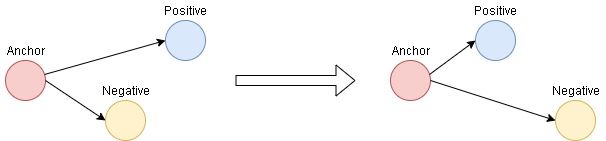
\includegraphics[scale=0.4]{img/TripletLoss.png}
	\caption{Triplet Loss}
	\label{fig:Triplet}
\end{figure}

\section{CycleGAN}
\vspace{1ex}

\begin{figure}  [!htb]
	        \captionsetup{justification=centering}
	        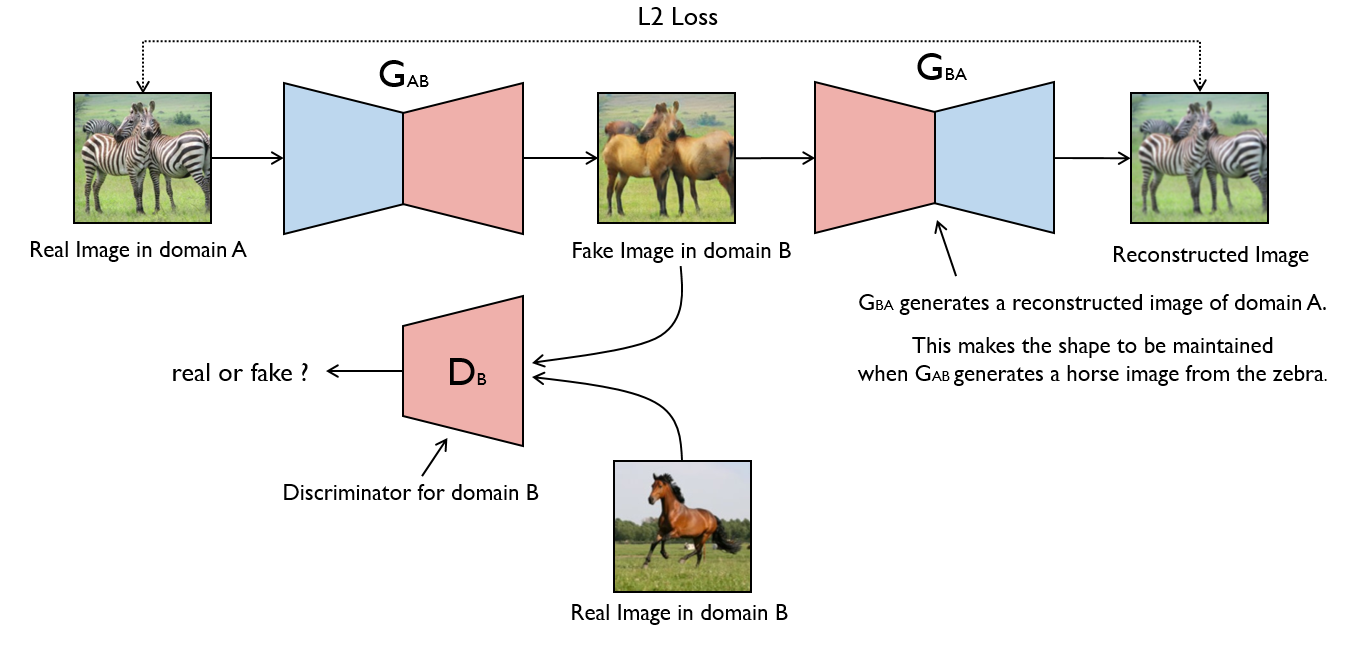
\includegraphics[scale=0.2]{img/cyclegan.png}
	        \caption{CycleGAN}
	        \label{fig: 3_18}
\end{figure}

CycleGAN merupakan sebuah teknik yang menggunakan \textit{Deep Convolutional Neural Network} untuk melakukan sinstesis sebuah gambar versi baru dengan modifikasi yang diinginkan, seperti mengubah gambar dari musim panas ke musim salju. Pada umumnya \textit{training} model untuk melakukan hal tersebut membutuhkan dataset dengan contoh berpasangan(\textit{paired example}) yang sangat besar. Cara seperti ini membutuhkan waktu yang sangat lama, dan pada beberapa kasus tertentu tidak dapat dilakukan. Namun dengan menggunakan CycleGAN, model dapat secara otomatis melakukan \textit{training} untuk translasi \textit{Image-to-image}.  dilatih secara \textit{unsupervised} dengan menggunakan kumpulan gambar dari sebuah domain X ke sebuah domain Y, tanpa harus memasangkan kedua gambar tersebut.

\section{\textit{Local Binary Pattern}}
\vspace{1ex}

\begin{figure}  [!htb]
	        \captionsetup{justification=centering}
	        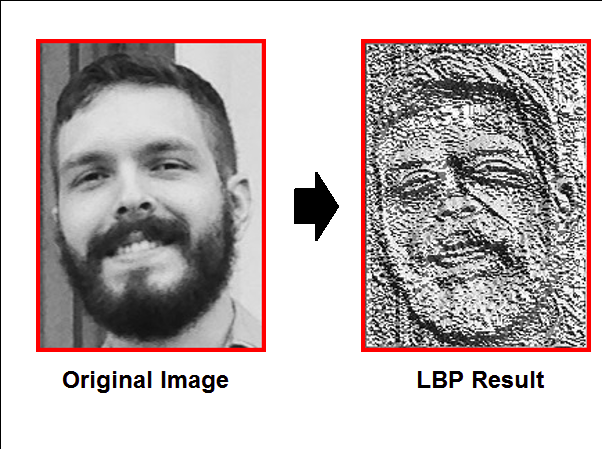
\includegraphics[scale=0.2]{img/lbp.png}
        	%\caption{Diagram alur kerja}
        	\caption{Local Binary Pattern}
        	\label{fig: 3_27}
\end{figure}

\textit{Local Binary Pattern} (LBP) merupakan salah satu deskriptor visual yang digunakan pada visi komputer. Pada umumnya LBP digunakan pada Face Recognition dikarenakan LBP merupakan deskriptor yang sangat kuat untuk melakukan klasifikasi tekstur. Selain itu telah ditemukan bahwa ketika LBP digabungkan dengan deskriptor \textit{Histogram of Oriented Gradients} (HOG), performa yang didapatkan bertambah secara drastis pada beberapa dataset tertentu.

\par Cara kerja dari LBP sendiri adalah sebagai berikut:
\begin{enumerate}
	\vspace{-2mm}
	\item Ubah citra menjadi bentuk \textit{grayscale} / hitam putih.
	\vspace{-2mm}
	\item Bagi citra menjadi beberapa bagian(\textit{cell})
	\vspace{-2mm}
	\item Untuk setiap \textit{pixel} yang terdapat pada sebuah \textit{cell}, bandingkan dengan pixel milik 8 neighbor yang terdapat di sekelilingnya
	\vspace{-2mm}
	\item Apabila nilai dari pixel yang di tengah lebih besar dari setiap pixel pada neighbornya maka pixel tersebut diberi nilai 0, selain itu pixel tersebut diberi nilai 1.
	\vspace{-2mm}
	\item Hitung Histogram
	\vspace{-2mm}
	\item Normalisasi Histogram.
\end{enumerate}
